\subsection{Categorical data require different graphical methods}\label{sec:intro-catdata}

We will see in Chapters 6--7 that statistical models for discrete
response data and for frequency 
data are close analogs of the linear regression and ANOVA models
used for quantitative data.
These analogies suggest that the graphical methods
commonly used for quantitative data may be adapted directly to
categorical data.

Happily, it turns out that many of the analysis graphs and diagnostic
displays (e.g., influence plots, added variable and partial residual
plots, etc.)
which have become common adjuncts in the analysis of
quantitative data have been extended to generalized linear models
including logistic regression and \loglin\ models.

Unhappily, the familiar techniques for displaying raw data are
often disappointing when applied to categorical data.
The simple \scat, for example, is widely used to show
the relation between
quantitative response and predictors, together with the fitted linear
model.
For the arthritis data in case form (\datref{dat:arthrit})
the analogous plot for a logistic regression model
(predicting Pr(Some or Marked) improvement from Age) shown in the
left panel of \figref{fig:logist1c0}, is, well,  underwhelming.
First, the response, Improve, takes on only the values 0 and 1,
and Age (in years) is also discrete, so many points overplot
in this graph.%
\footnote{Only 51 distinct points are shown for the 84 observations.}
Second, although this graph is enhanced with the curve of predicted
probabilities under the fitted model (solid line) and 95\% confidence
bands (dashed lines), it is hard to appreciate how the data points
relate to the fitted model.  (Can you see that the probability of
improvement increases with age?)
%% two subfig side-by-side
\begin{figure}[htb]
 \begin{minipage}[c]{.49\linewidth}
  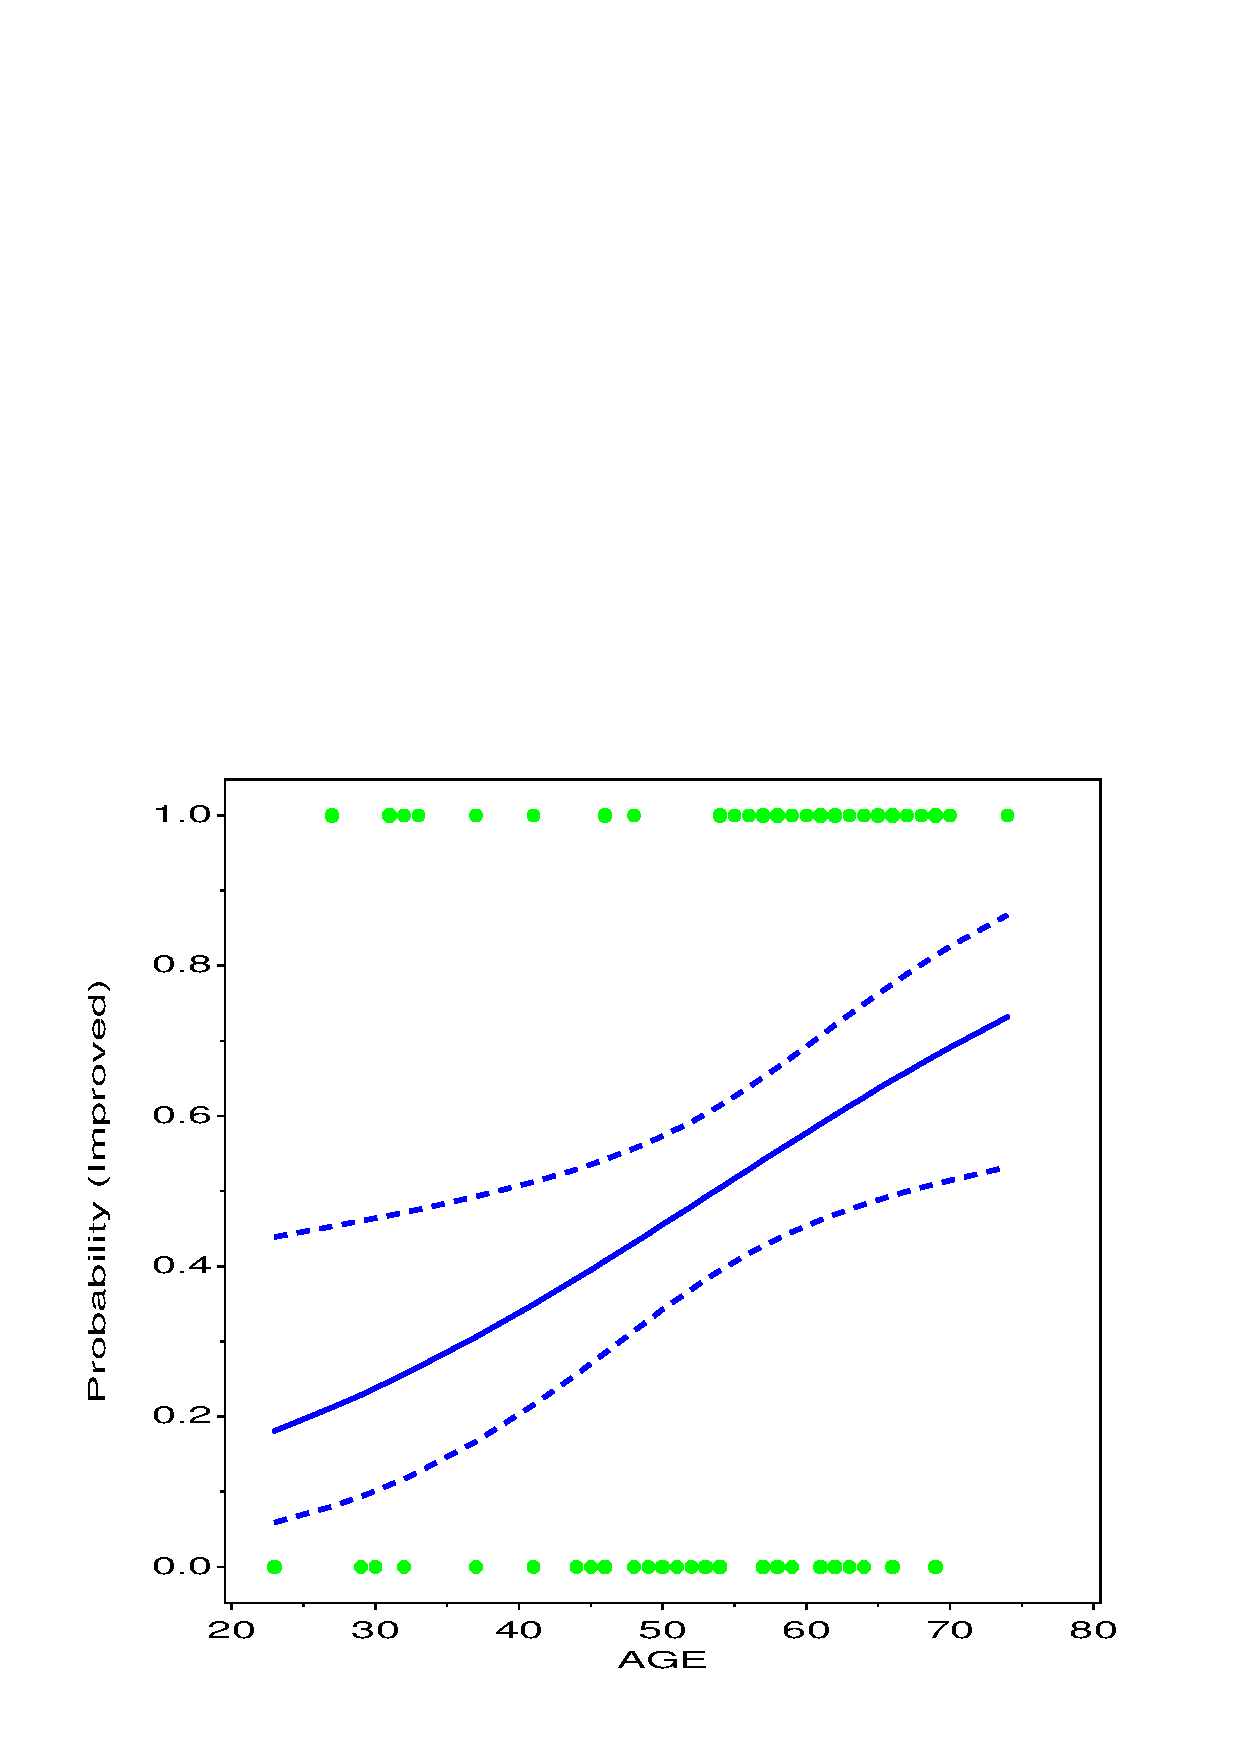
\includegraphics[width=1\linewidth,clip]{ch1/fig/logist1c0}
 \end{minipage}%
 \hfill
 \begin{minipage}[c]{.49\linewidth}
  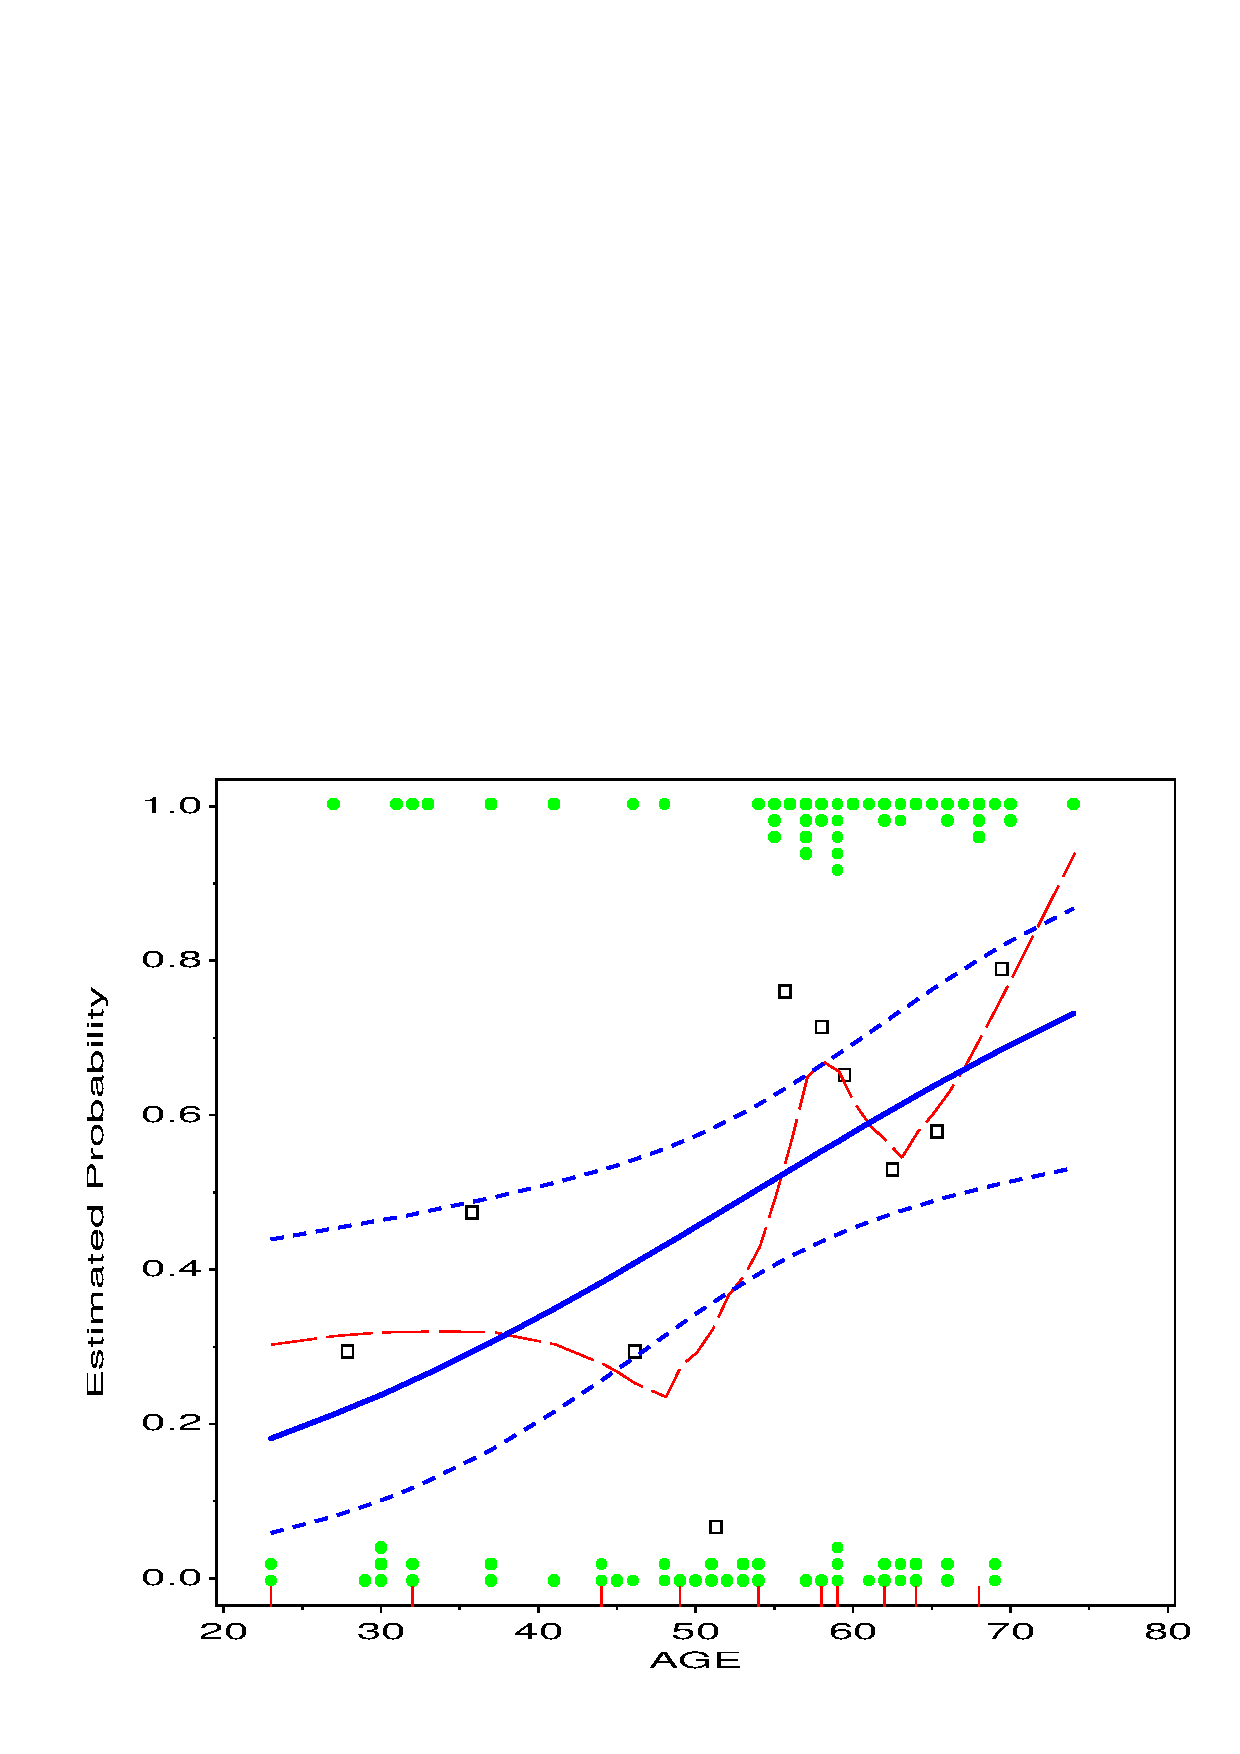
\includegraphics[width=1\linewidth,clip]{ch6/fig/logoddt2}
 \end{minipage}
 \caption[Graphical displays for Arthritis treatment data]{Graphical displays for Arthritis treatment data. Left: raw data
 with logistic regression on age; right: stacked raw data, logistic regression, and smoothed lowess curve.}\label{fig:logist1c0}
\end{figure}


These problems may be reduced to some degree by smoothing and by
jiggling the points to avoid overplotting.
The right panel of \figref{fig:logist1c0} shows a modest improvement.
Here, the raw observations were offset by stacking down from 1 and up
from 0 wherever duplicate observations occurred.
In addition, the observations were grouped into tenths by age; the lower
boundaries of the age categories are shown by the tick marks on the horizontal
scale.  The proportion of Improved responses in each age group is then
plotted (squares), and a non-parametric (lowess) smoothed curve is added
to the plot.
Although the smoothed curve is somewhat jagged, we now have a clearer
visual impression that the probability of improvement increases with age,
and we can see the large number of 1 responses among older people.

In \figref{fig:logist1c0} the quantitative variable Age supports
the use of the \scat\ as the graphic format for visual display. 
A more essential difference between quantitative data and categorical
data arises when all variables are categorical, as in a \ctab\
like \tabref{tab:arthrit0}.   Then, we find that a different visual
representation is more natural and useful
\citep{Friendly:95,Friendly:97}.  

For quantitative data, magnitude can
be represented by length (in a bar chart) or by position along a
scale (dotplots, scatterplots).  When the data are purely categorical,
design principles of perception, detection, and comparison
\citep{Friendly:99} suggest that frequencies are most usefully
represented as areas.  In spite of the fact that
(in magnitude estimation tasks) judgments of
area are known to be less accurate than those of length
(e.g., \citet{ClevelandMcGill:84b}), there
are two fundamental reasons why area is a preferred visual representation
for count data:
\begin{itemize}
\item multiplicative relations of probabilities and expected frequencies
translate readily into height and width of rectangles, whose area then
depicts a cell value.

\item a concrete, physical model for categorical data \citep{Friendly:95}
based on count $\sim$ area 
yields a surprising range of correct, but novel
interpretations for statistical principles (maximum likelihood),
estimation techniques (iterative proportional fitting, Newton--Raphson)
and statistical concepts (power, why components of likelihood-ratio $G^2$ can be
negative).
\end{itemize}

\ix{sieve diagram|(}
The first point is illustrated in \figref{fig:sievebrk1},
a sieve diagram (\secref{sec:twoway-sieve})
for the Berkeley admissions data, broken down by department.
In this display, each box has a height proportional to the marginal total
for the corresponding department and width proportional to the column
marginal total, so the area is proportional to the expected frequency
under independence.  The observed frequency in each cell is shown
by the number of cross-ruled boxes, so departures from independence
are shown visually as variations in shading density.
\begin{figure}[htb]
  \centering
  \includegraphics[scale=.6]{ch1/fig/sievebrk1}
  \caption[Sieve diagram for Berkeley admissions data]{Sieve diagram for Berkeley admissions data.  Each box has area proportional to its expected frequency, and is cross-ruled with boxes equal to the observed frequency.}\label{fig:sievebrk1}
\end{figure}
\ix{sieve diagram|)}

The second point is illustrated in \figref{fig:mosdemo},
using data (see \tabref{tab:hairdat}) on $n=592$ individuals
classified by hair color.
In the conceptual model
\citep{Friendly:95,Sall:91b}, categorical observations are likened to
molecules of an ideal gas confined to chambers separated by moveable
partitions.  In both panels of the figure, the number of symbols in each box exactly
equals the number of observations in each hair color category.

%% two subfig side-by-side
\begin{figure}[htb]
 \begin{minipage}[t]{.49\linewidth}
  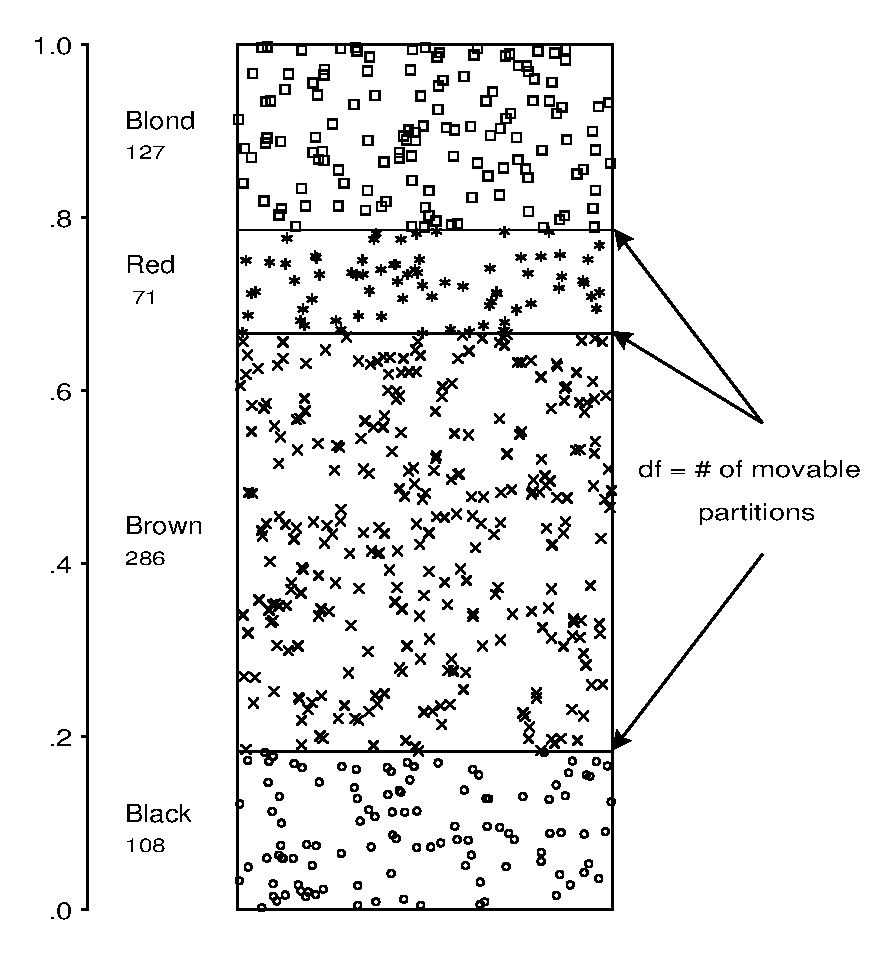
\includegraphics[width=1\linewidth,clip]{ch1/fig/mosdemo3}
 \end{minipage}%
 \hfill
 \begin{minipage}[t]{.49\linewidth}
  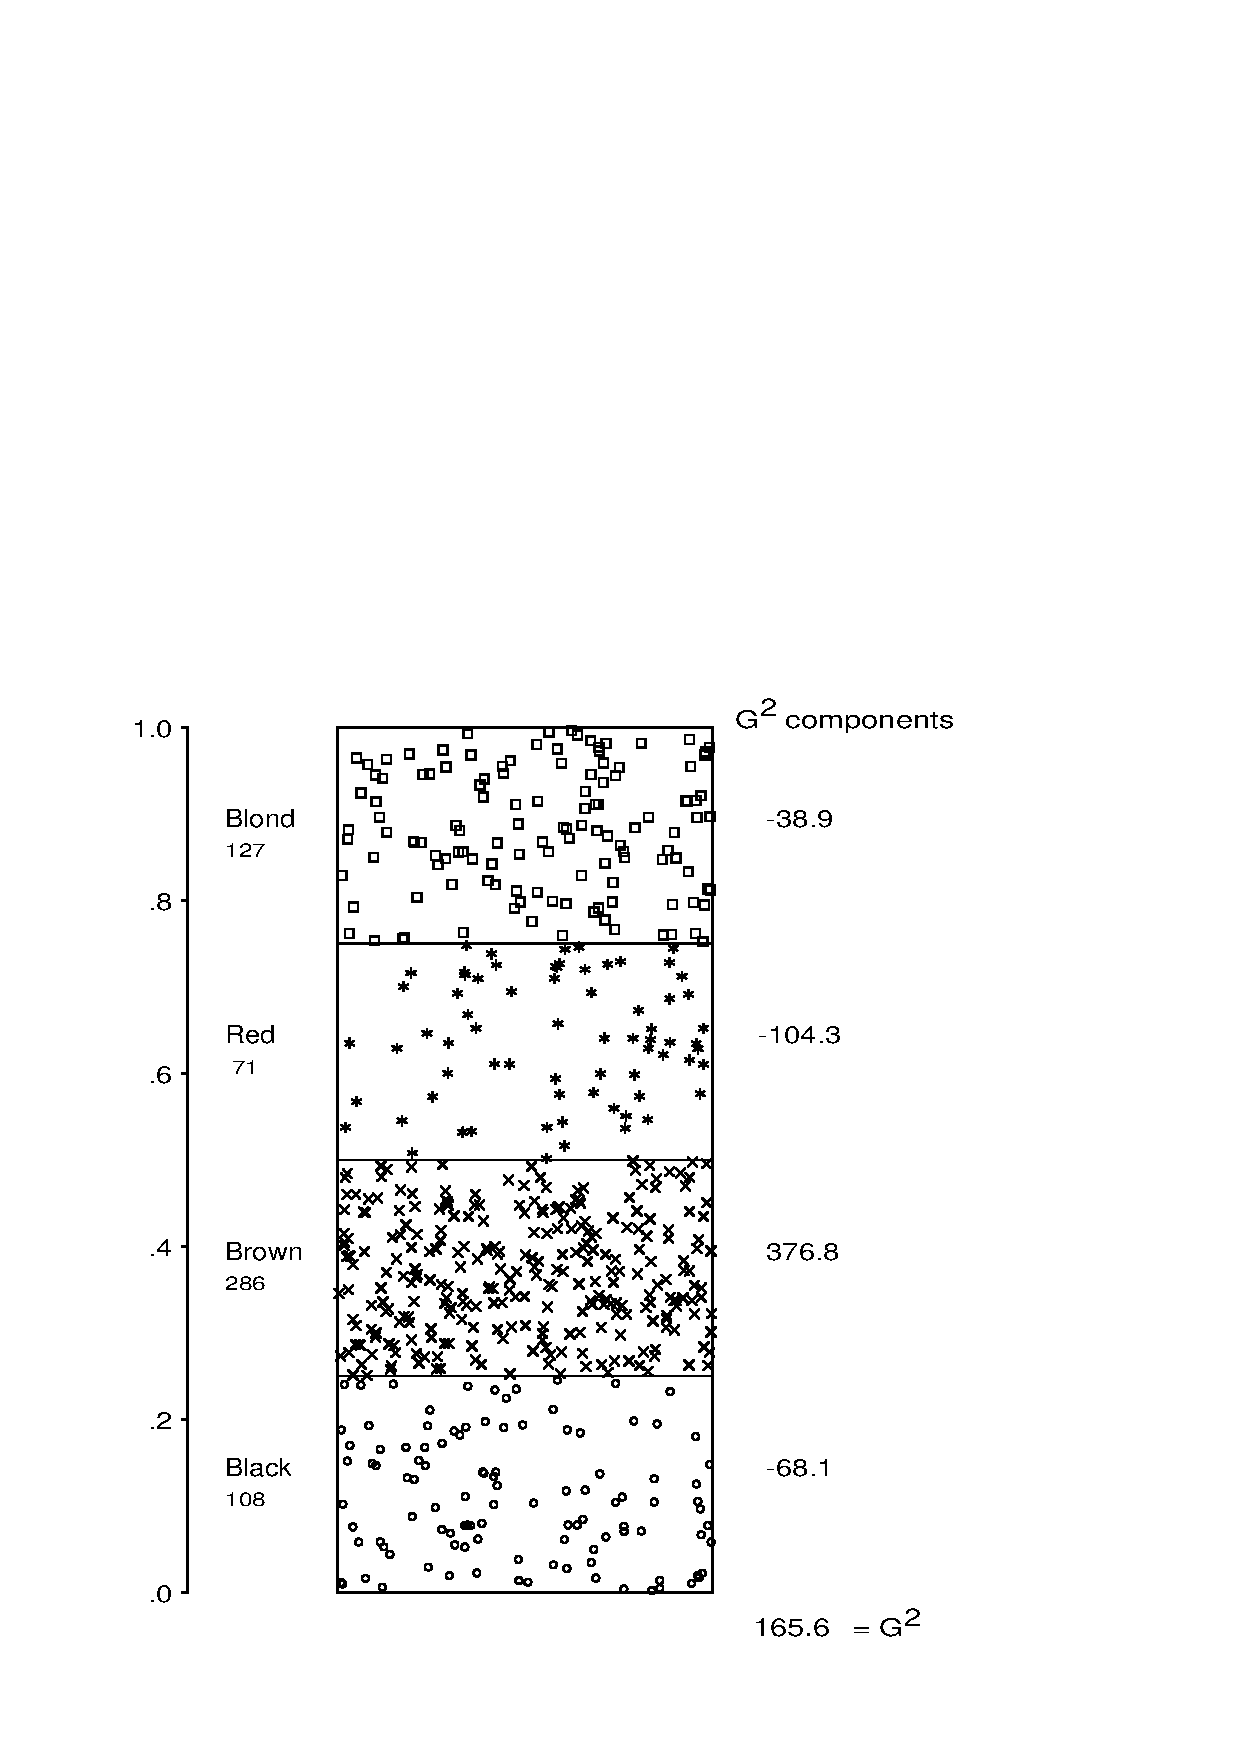
\includegraphics[width=1\linewidth,clip]{ch1/fig/mosdemo4}
 \end{minipage}
 \caption{Conceptual model for categorical data}\label{fig:mosdemo}
\end{figure}

When the location of the partitions are unconstrained, as in the
left panel of \figref{fig:mosdemo}, the forces balance in each chamber
by moving to the positions of minimum potential energy, so that
the height of each chamber is $p_i = n_i / n$, which is the maximum likelihood
estimate of the probability $\pi_i$ in each cell.

To test the hypothesis that all hair colors are equally likely,
imagine forcing the partitions to move to the positions where
$\pi_i = \frac{1}{4}$, as shown in the right panel.
The change in energy in each compartment is then 
$- ( \log  p_i - \log  \pi_i ) = - \log ( p_i / \pi_i )$ , 
the change in negative log-likelihood. Sum these up and multiply by 2 to get the likelihood ratio \GSQ. This gives a concrete interpretation of \GSQ\ as a measure of the effort to maintain belief in the hypothesis in the face of the data. 

This concrete model supplies neat explanations of many other results for categorical data, extends readily to multiway tables, and provides a rationale for the graphic representation of counts by area or visual density.
It also serves as basis for the mosaic display, described in
\chref{ch:mosaic}.
